

\subsection{Arbre exponentiel}
\label{repl:subsec:exponentialtree}

Un arbre exponentiel est une structure d'arbre dont chacun des nœuds possède une
arité maximale $k$ fois supérieure à celle de son parent. Ainsi, si $k$ est fixé
à 2 et que la racine peut accueillir 8 fils, alors chacun de ces fils peut
accueillir à son tour 16 fils etc. Ainsi, la progression du nombre de fils dans
une branche est exponentielle.

\TODO{Moar.}

\begin{figure}
  \centering
  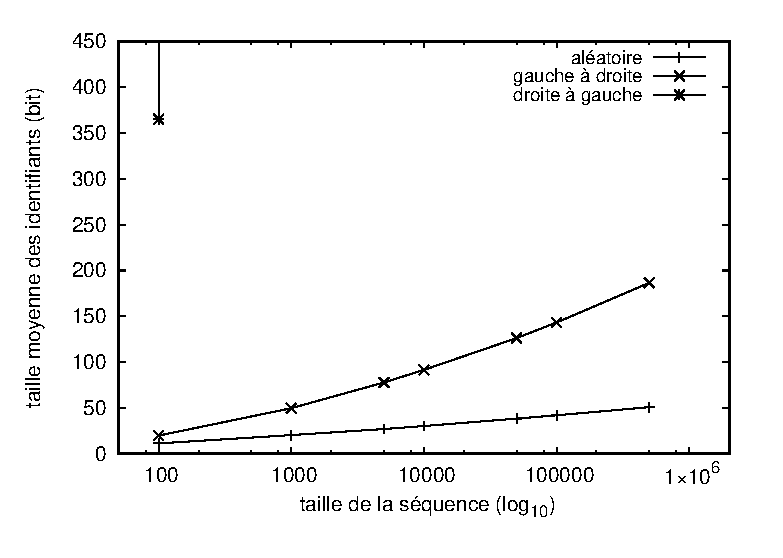
\includegraphics[width=0.8\textwidth]{img/lseq/double.eps}
  \caption{\label{repl:img:exponentialtree} Arbre exponentiel avec stratégie
    d'allocation adaptée à l'édition en fin. L'axe des abscisses montre la
    taille du document sur une échelle logarithmique en base décimale. L'axe des
    ordonnées montre la moyenne des tailles des chemins alloués.}
\end{figure}

\begin{itemize}
\item [\textbf{Objectif :}] Montrer que le chemin des identifiants alloués
  progresse de manière sous-linéaire par rapport à la taille du
  document. Montrer que lorsque le comportement d'édition va à l'opposé de celui
  prévu, l'allocation devient désastreuse.
\item [\textbf{Description :}] Des documents sont créés artificiellement par
  insertions successives de caractères. Trois types de comportement d'édition
  sont simulés :
  \begin{inparaenum}[(i)]
  \item à des positions aléatoire dans le document,
  \item à la fin,
  \item en tête.
  \end{inparaenum}
  La moyenne de la taille des identifiants est mesurée à 100, 1k, 5k, 10k, 50k,
  100k, 500k insertions. La structure utilisée est celle d'un arbre exponentiel
  dont l'arité maximale de départ est fixée à $2^5$.
\item [\textbf{Résultat :}] La figure~\ref{repl:img:exponentialtree} montre les
  résultats des mesures effectuées pendant la simulation. Nous observons que
  lors de l'édition en position aléatoire, l'allocation se comporte extrêmement
  bien avec des chemins de taille logarithmique. Lors de l'édition en fin, la
  taille moyenne des chemins suit une augmentation sous-linéaire par rapport au
  nombre d'insertions dans le document. Finalement, l'édition en tête entraine
  une très forte augmentation de la taille des identifiants.
\item [\textbf{Explication :}] L'édition aléatoire place les éléments au hazard
  dans la séquence. L'arbre est équilibré car nulle branche n'est remplie en
  particulier. À terme, toutes les branches les plus basses sont remplies. Dans
  ce cas, les chemins sont de taille moyenne logarithmiques ce qui constitue la
  borne minimale. Lors de l'édition en queue, les chemins les plus à gauche sont
  alloués réservant de l'espace aux insertions futures. De plus, puisque l'arité
  de l'arbre double à chaque niveau, il peut accueillir deux fois plus de
  chemins à un prix minime (+1 bit/niveau). Pour cette même raison, l'allocation
  est désastreuse lors de l'édition en tête : Quelques insertions suffisent à
  faire augmenter la profondeur de l'arbre. L'arité maximale augmente alors
  rapidement et le prix des identifiants explose.
\end{itemize}


%%% Local Variables:
%%% mode: latex
%%% TeX-master: "../../paper"
%%% End:
